\documentclass[aspectratio=169]{beamer}
\usetheme[block=fill]{metropolis}
\usepackage{tikz}
\usetikzlibrary{shapes.geometric, arrows.meta, positioning, calc}

\title{Building a Reproducible Scholarly Search Toolkit}
\subtitle{Episode 20: Publishing to PyPI}
\author{Scholar Search Kit}
\date{}

\begin{document}

\begin{frame}[plain]
  \titlepage
\end{frame}

\begin{frame}{Episode Goal}
  \begin{alertblock}{The Goal}
    Prepare our \texttt{pyproject.toml} and publish the library to the Python Package Index (PyPI) so anyone can \texttt{pip install} it.
  \end{alertblock}
  \vspace{0.5cm}
  Code that sits on your hard drive isn't a tool; it's a script. Publishing makes it accessible to the global research community.
\end{frame}

\begin{frame}{The \texttt{pyproject.toml} Metadata}
  \begin{block}{The Manifest}
    Modern Python packages use \texttt{pyproject.toml} instead of \texttt{setup.py}.
  \end{block}
  
  \begin{itemize}
      \item \textbf{Dependencies:} We list \texttt{httpx} and \texttt{pydantic} so \texttt{pip} installs them automatically.
      \item \textbf{Scripts:} We define \texttt{scholar-search = "scholar\_search.cli:main"} to create a global terminal command.
      \item \textbf{Metadata:} Authors, URLs, and Open Source Licenses.
  \end{itemize}
\end{frame}

\begin{frame}{The Build Process}
  \begin{center}
  \resizebox{0.6\linewidth}{!}{
  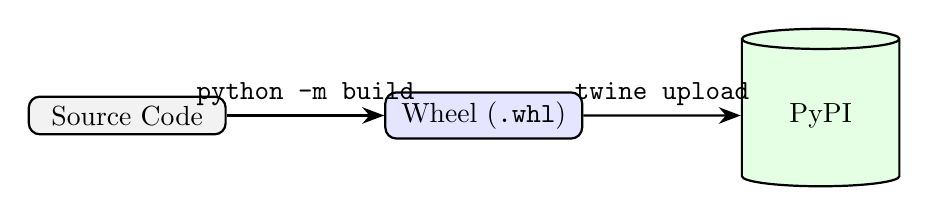
\begin{tikzpicture}[
      node distance=1.5cm and 2cm,
      src/.style={rectangle, draw, thick, rounded corners, minimum width=2.5cm, align=center, fill=black!5},
      build/.style={rectangle, draw, thick, rounded corners, minimum width=2.5cm, align=center, fill=blue!10},
      pypi/.style={cylinder, draw, thick, shape border rotate=90, aspect=0.25, minimum height=2cm, minimum width=2cm, align=center, fill=green!10},
      arrow/.style={-{Stealth[scale=1.2]}, thick}
    ]
    
    \node[src] (s) {Source Code};
    \node[build, right=of s] (b) {Wheel (\texttt{.whl})};
    \node[pypi, right=of b] (p) {PyPI};
    
    \draw[arrow] (s) -- node[above] {\texttt{python -m build}} (b);
    \draw[arrow] (b) -- node[above] {\texttt{twine upload}} (p);
  \end{tikzpicture}
  }
  \end{center}
  \vspace{0.2cm}
  We convert our raw Python files into a zipped \texttt{Wheel} format, which is heavily optimized for fast installation.
\end{frame}

\begin{frame}{Verification}
  \begin{alertblock}{Success Criteria}
    \begin{itemize}
        \item Running \texttt{python -m build} succeeds without errors.
        \item The resulting \texttt{.whl} file can be installed into a fresh virtual environment.
        \item Typing \texttt{scholar-search --help} works globally on the system.
    \end{itemize}
  \end{alertblock}
\end{frame}

\end{document}
